\documentclass[12pt]{article}

\usepackage{sbc-template}
\usepackage{graphicx,url}
\usepackage[brazil]{babel}
\usepackage[utf8]{inputenc}
\usepackage{float}
\usepackage{setspace}

\usepackage{tabularx}
\usepackage{cite}

\sloppy

\title{Detecção de Alertas de Seguranças em Redes de Computadores Usando o
Internet Relay Chat}

\author {Daniel C. Bucher\inst{1}, Rodrigo Campiolo\inst{1,2}, Daniel M. Batista\inst{1} }


\address{Instituto de Matemática e Estatística -- Universidade de São Paulo (USP)\\
  Rua do Matão, 1010 - CEP 05508-090 - São Paulo - SP
\nextinstitute
  Universidade Tecnológica Federal do Paraná (UTFPR)\\
  Campo Mourão, PR -- Brasil
  \email{\{dbucher, batista\}@ime.usp.br, rcampiolo@utfpr.edu.br}
}

\begin{document}

\maketitle

\begin{resumo}
  Resumo.


\end{resumo}

\begin{abstract}
  Abstract.


\end{abstract}

%-----------------------------------------------------------------------------%
\section{Introdução} \label{sec:intro}

Introdução será escrita por último.

%-----------------------------------------------------------------------------%
\section{Trabalhos Relacionados} \label{sec:rel}

%TODO Internet Relay Chat deveria permanecer em itálico?
Nesta seção, apresentamos alguns trabalhos relacionados. Os trabalhos são
divididos em dois tipos. O primeiro consiste em trabalhos que procuram usar fontes de
dados abertas para detectar alertas de problemas de segurança em redes de
computadores. O segundo tipo consiste em trabalhos que buscam realizar algum
tipo de investigação em ferramentas de chat.

\citeonline{santos2013} apresentaram um método de extração de notificações de
segurança de redes de computadores a partir de mensagens postadas na rede de
\textit{microblogging}, Twitter.
%
A metodologia apresentada nesse trabalho, consiste em coletar mensagens
postadas no Twitter e processar essas mensagens usando as técnicas de
agrupamento e classificação. Na seção \ref{sec:metod} descrevemos essas duas
técnicas, uma vez que utilizaremos as mesmas neste trabalho.
%
A combinação dessas técnicas obteve uma precisão de 92\% de mensagens
que continham tópicos relacionados à segurança de redes, e 50\% que
representavam potenciais alertas.

No que diz respeito ao IRC, a maioria dos trabalhos encontrados por nós
realizam uma análise \textit{post mortem} de logs contendo as mensagens de
determinado canal.
%
Existem poucos trabalhos que buscam fazer algum tipo de análise em tempo real,
ou quase em tempo real, de mensagens na rede.
%
Em sua dissertação de mestrado, \citeonline{brown2007} propõe uma arquitetura para
uma ferramenta de investigação automática no IRC. A arquitetura proposta
consiste em cinco módulos: (\textit{i}) o módulo de coleta responsável por
capturar as mensagens e realizar um \textit{parse} em busca de datas, nomes
de usuário e \textit{hyperlinks};
%
(\textit{ii}) o módulo de armazenamento
salva as mensagens e eventos, como entrada e saída de usuários em canais, em
um banco de dados;
%
(\textit{iii}) o módulo de análise verifica se existem referências à atividades
criminosas nas mensagens;
%
(\textit{iv}) o módulo de alerta recupera os dados do módulo de análise e envia,
por correio eletrônico e mensagens de texto no celular, para as autoridades responsáveis;
%
e por fim, (\textit{v}) o módulo localizador tenta rastrear a origem dos
usuários remetentes das mensagens. Para tanto, ele utiliza o comando \textbf{WHOIS} do
protocolo do IRC. No entanto, Brown avisa que esse módulo pode não
retornar informação relevante.
%
A análise das mensagens é realizada utilizando as técnicas de análise de
palavras chave e análise de bancos de dados \cite{brown2007}.
%
Essa abordagem, no entanto, requer que o investigador saiba com antecedência
quais canais monitorar.

\citeonline{michels2012} propôs uma ferramenta de análise em tempo real de
conversas no IRC. Seu trabalho difere da abordagem dos demais trabalhos
encontrados na literatura pois adiciona um módulo de \textit{crawlers} para
auxiliar o investigador a encontrar os canais a serem monitorados.
%
Esse módulo funciona em duas etapas. A primeira consiste no que ele chama de
\textit{topic crawler}, ele realiza a análise de palavras chave nos nomes e
nas descrições de todos os canais de determinado servidor. A seguir, um
\textit{channel crawler} entra nos canais identificados e escuta as conversas
por um curto período de tempo e realiza a análise de palavras chaves de forma
a identificar com maior precisão se o canal deve ser marcado para revisão do
investigador.

A análise das mensagens foi realizada de duas formas. Primeiramente era
realizada tanto a análise de palavras chave por si só, quanto a análise de
palavras chave combinada com a análise de \textbf{\textit{Part of Speech
Tagging} (POST)} \cite{stanford}. A análise POST quebra a frase em partes e
define as classes gramaticais de cada parte. No entanto, \citeonline{michels2012}
observou que o uso desse tipo de análise não produz diferenças significativas,
se comparado com o uso de análise de palavras chave sozinho.

O segundo tipo de análise foi a análise de tópico quase em tempo real.
\citeonline{michels2012} implementou o método de análise \textit{classic frequency}
\cite{gainaru2010} pois ele é facilmente adaptável para uma ferramenta que analisa
dados em tempo real.
%
Michels ressalta que no geral, análises de tópico são realizadas em logs
após a coleta dos dados. Para simular esse efeito, ele definiu um limite de
mensagens de forma que a análise de tópicos só era realizada após o módulo de
coleta ter coletado esse limite.
%
A conclusão foi de que o tópico de análise não funciona bem porque as
ferramentas utilizadas para \textit{stemming} (processo de reduzir uma
palavra derivada à palavra raiz que a originou), \textit{thesaurus}, etc.
não estão preparadas para analisar jargões e gírios, comuns quando se trata
de comunicação através da internet.

\begin{figure}[ht]
\centering
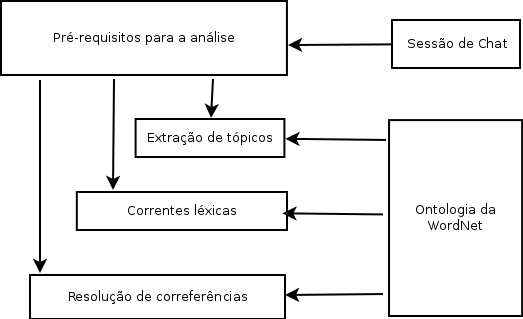
\includegraphics[width=.6\textwidth]{images/gainaru_architecture.png}
\caption{Arquitetura do \textit{toolkit} apresentado por \cite{gainaru2010}}
\label{fig:gainaru-architecture}
\end{figure}

\citeonline{gainaru2010} afirmam que as ferramentas
de análise de texto não levam em consideração a estrutura temporal que
fontes de dados baseadas em conversas de chat possuem. Eles então apresentaram
um \textit{toolkit} para análise automática de conversas em chats.
%
A \ref{fig:gainaru-architecture} apresenta a arquitetura proposta por por eles.
Essa arquitetura é dividida em quatro módulos.

O primeiro, realiza alguns procedimentos que atuam como pré-requisitos para
a análise do texto. Esses procedimentos são:
%
(\textit{i}) \textit{tokenização}, que consiste em separar as frases em
palavras individuais;
%
(\textit{ii}) eliminação de palavras sem relevância, por exemplo
\textit{emoticons} como ':)';
%
(\textit{iii}) \textit{word stemming}, que consiste em extrair a forma raiz
de uma palavra;
%
e por último, (\textit{iv}) a análise POST citada anteriormente.
%
O segundo módulo busca extrair um ou mais tópicos de uma conversa. Para
tanto, eles realizam uma análise de frequência chamada de \textit{classic
frequency}, e agrupam palavras que são sinônimos. 
%
O resultado é considerado a lista de tópicos da conversa.
%
O terceiro módulo identifica correntes léxicas no texto. Uma corrente
léxica é uma lista de palavras que captura uma porção da estrutura 
coerente  do texto.
%
O quarto e último módulo analisa o texto em busca de correferências de
termos não verbais.

Na seção \ref{sec:metod}, apresentamos a metodologia adotada por nós, que
é uma combinação da metodologia utilizada por \cite{santos2013} e
\cite{michels2012} e que utiliza algumas técnicas apresentadas por
\cite{gainaru2010}.



%-----------------------------------------------------------------------------%
\section{Metodologia} \label{sec:metod}

Nesta seção, nós propomos uma metodologia para extrair e evidenciar alertas
relacionados a segurança de redes de computadores em canais do IRC. A
metodologia consiste em uma junção da metodologia utilizada para extrair
alertas de segurança de redes sociais proposta em \cite{santos2013} e na
metodologia para análise de textos em tempo real em conversas do IRC proposta
por \cite{michels2012}.

\cite{santos2012, campiolo2013} comprovaram que existem mensagens sobre ameaças
computacionais postadas no Twitter.
%
Apesar do IRC não ser mais a principal ferramenta de chat, ela
sobreviveu ao uso do tempo desde o final dos anos 80, e continua muito
utilizada por grupos de \textit{hackers} e empresas que trabalham com
tecnologia da informação. Em seu trabalho, por exemplo, \citeonline{michels2012}
observa que empresas podem detectar falhas em seus produtos mais rapidamente
se monitorarem alguns canais no IRC.

Nesse contexto, definimos duas questões de pesquisa para para extrair
efetivamente notificações de segurança obtidas de conversas em canais do IRC:

\begin{itemize}
	\item[\textbf{Q1}] O IRC consiste em uma fonte de informação relevante para se
	extrair alertas de segurança em redes de computadores?
	\item[\textbf{Q2}] É possível extrair e analisar informação relevante sobre alerta
	de segurança em redes de computadores de canais do IRC em tempo real, ou 
	quase real?
\end{itemize}

O método proposto por nós é composto por cinco etapas:

\begin{enumerate}

	\item Obter uma lista de canais que possam conter informação relevante.
	\item Obter as mensagens de segurança trocadas nos canais.
	\item Filtrar mensagens: remover mensagens que fogem ao contexto.
	\item Agrupar por similaridade: relacionar mensagens que relatam um mesmo
	assunto.
	\item Gerar lista de tópicos mais relevantes: detectar quais são os
	principais tópicos abordados nos canais.
\end{enumerate}

As subseções a seguir detalham cada uma dessas cinco etapas.

\subsection{Obter lista de canais}

(Canais com senha foram ignorados. A abordagem foi mista, \textit{crawlers}
mais seleção manual de alguns canais.) ...

\subsection{Obter mensagens}

...

%-----------------------------------------------------------------------------%
\section{Resultados} \label{sec:res}

Escreva os resultados aqui.

%-----------------------------------------------------------------------------%
\section{Discussão} \label{sec:disc}

Escreva os resultados aqui.


%-----------------------------------------------------------------------------%
\section{Conclusão e Trabalhos Futuros} \label{sec: concl}

Escreva a conclusão aqui.

\bibliographystyle{sbc}
\bibliography{paper}
\end{document}
